%%%%%%%%%%%%%%%%%%%%%%%%%%%%%%%%%%%%%%%%%%%%%%%%%%%%%%%%%%%%%%%
%
% Welcome to writeLaTeX --- just edit your LaTeX on the left,
% and we'll compile it for you on the right. If you give 
% someone the link to this page, they can edit at the same
% time. See the help menu above for more info. Enjoy!
%
%%%%%%%%%%%%%%%%%%%%%%%%%%%%%%%%%%%%%%%%%%%%%%%%%%%%%%%%%%%%%%%

% --------------------------------------------------------------
% This is all preamble stuff that you don't have to worry about.
% Head down to where it says "Start here"
% --------------------------------------------------------------
 
\documentclass[14pt]{article}
 
\usepackage[margin=0.5in]{geometry} 
\usepackage{amsmath,amsthm,amssymb}
\usepackage{graphicx}
\usepackage{subcaption}
%\usepackage{hyperref}
\usepackage{color,soul}
\usepackage{caption}
\usepackage{courier}
\usepackage{float}
\usepackage{listings}
\usepackage{xcolor} % for setting colors
\usepackage[bookmarksnumbered=true, citebordercolor={1 0 0}]{hyperref} 
\usepackage[title]{appendix}
\hypersetup{colorlinks=true, linkcolor=blue,urlcolor=blue}

\newcommand{\N}{\mathbb{N}}
\newcommand{\Z}{\mathbb{Z}}

\newenvironment{theorem}[2][Theorem]{\begin{trivlist}

\item[\hskip \labelsep {\bfseries #1}\hskip \labelsep {\bfseries #2.}]}{\end{trivlist}}
\newenvironment{lemma}[2][Lemma]{\begin{trivlist}
\item[\hskip \labelsep {\bfseries #1}\hskip \labelsep {\bfseries #2.}]}{\end{trivlist}}
\newenvironment{exercise}[2][Exercise]{\begin{trivlist}
\item[\hskip \labelsep {\bfseries #1}\hskip \labelsep {\bfseries #2.}]}{\end{trivlist}}
\newenvironment{problem}[2][Problem]{\begin{trivlist}
\item[\hskip \labelsep {\bfseries #1}\hskip \labelsep {\bfseries #2.}]}{\end{trivlist}}
\newenvironment{question}[2][Question]{\begin{trivlist}
\item[\hskip \labelsep {\bfseries #1}\hskip \labelsep {\bfseries #2.}]}{\end{trivlist}}
\newenvironment{corollary}[2][Corollary]{\begin{trivlist}
\item[\hskip \labelsep {\bfseries #1}\hskip \labelsep {\bfseries #2.}]}{\end{trivlist}}

\newenvironment{solution}{\begin{proof}[Solution]}{\end{proof}}
\newenvironment{courier}{\ttfamily}{\par}

% set the default code style
\lstset{
    frame=tb, % draw a frame at the top and bottom of the code block
    tabsize=4, % tab space width
    showstringspaces=false, % don't mark spaces in strings
    numbers=left, % display line numbers on the left
    commentstyle=\color{orange}, % comment color
    keywordstyle=\color{blue}, % keyword color
    stringstyle=\color{red} % string color
}

\begin{document}
 
% --------------------------------------------------------------
%                         Start here
% --------------------------------------------------------------
 
\title{\textbf{General Hall C Analysis Procedure in 12 GeV Era}}%replace X with the appropriate number
\author{Carlos Yero \\ email \href{mailto:cyero002@fiu.edu}{cyero002@fiu.edu}} %if necessary, replace with your course title
 
\maketitle
\noindent The general Hall C analysis procedure for experiments in the 12 GeV era is discussed. The procedure
outlines the first necessary steps in the data analysis regardless of the nature of the experiment. These include, but are not
limited to: \\ \textit{1. reference time cuts}, \textit{2. detector time window cuts}, \textit{3. detector calibrations}.
Additional necessary procedures will be added in subsequent sections as updates to this document are made.

\section{Set Reference Time Cuts}\label{sec:ref_time_cuts}
\noindent The first step in Hall C Data Analysis is to make sure the \textit{reference time}  cuts are set properly,
as one needs to make sure the reference times correlated with the trigger are selected. The \textit{reference time}
is a copy of the pre-trigger which is distributed to all ADCs/TDCs in all detectors Read-Out Crontrollers (ROCs)\footnote{Refer to \url{https://hallcweb.jlab.org/DocDB/0010/001028/002/trigger_v2.pdf} for a detailed discussion on the Hall C trigger}. When the pre-trigger
is accepted, all crates read-out detector signals associated with the trigger, including the reference time itself (copy of pre-trigger). The
reference time is subtracted from the detector signal later on during the analysis replay. When using the reference time,
the Hall C analyzer, \textit{hcana}, choses the first hit in the time window if multiple hits are present per event. In this scenario, the first hit may NOT
necessarily be the \textit{good hit}, and the wrong reference time would be chosen resulting in the wrong time being subtracted in the ADC/TDC spectra.
By placing a reference time cut, the analyzer then considers the first hit after the cut, which is likely to be a \textit{good hit}. \\
\indent As an example, consider the H(e,e')p Elastic coincidence run 3377 which had the highest SHMS rate of elastics taken during the E12-10-003 experiment.

\begin{figure}[H]
  \centering
  \captionsetup{justification=raggedright,singlelinecheck=false}
  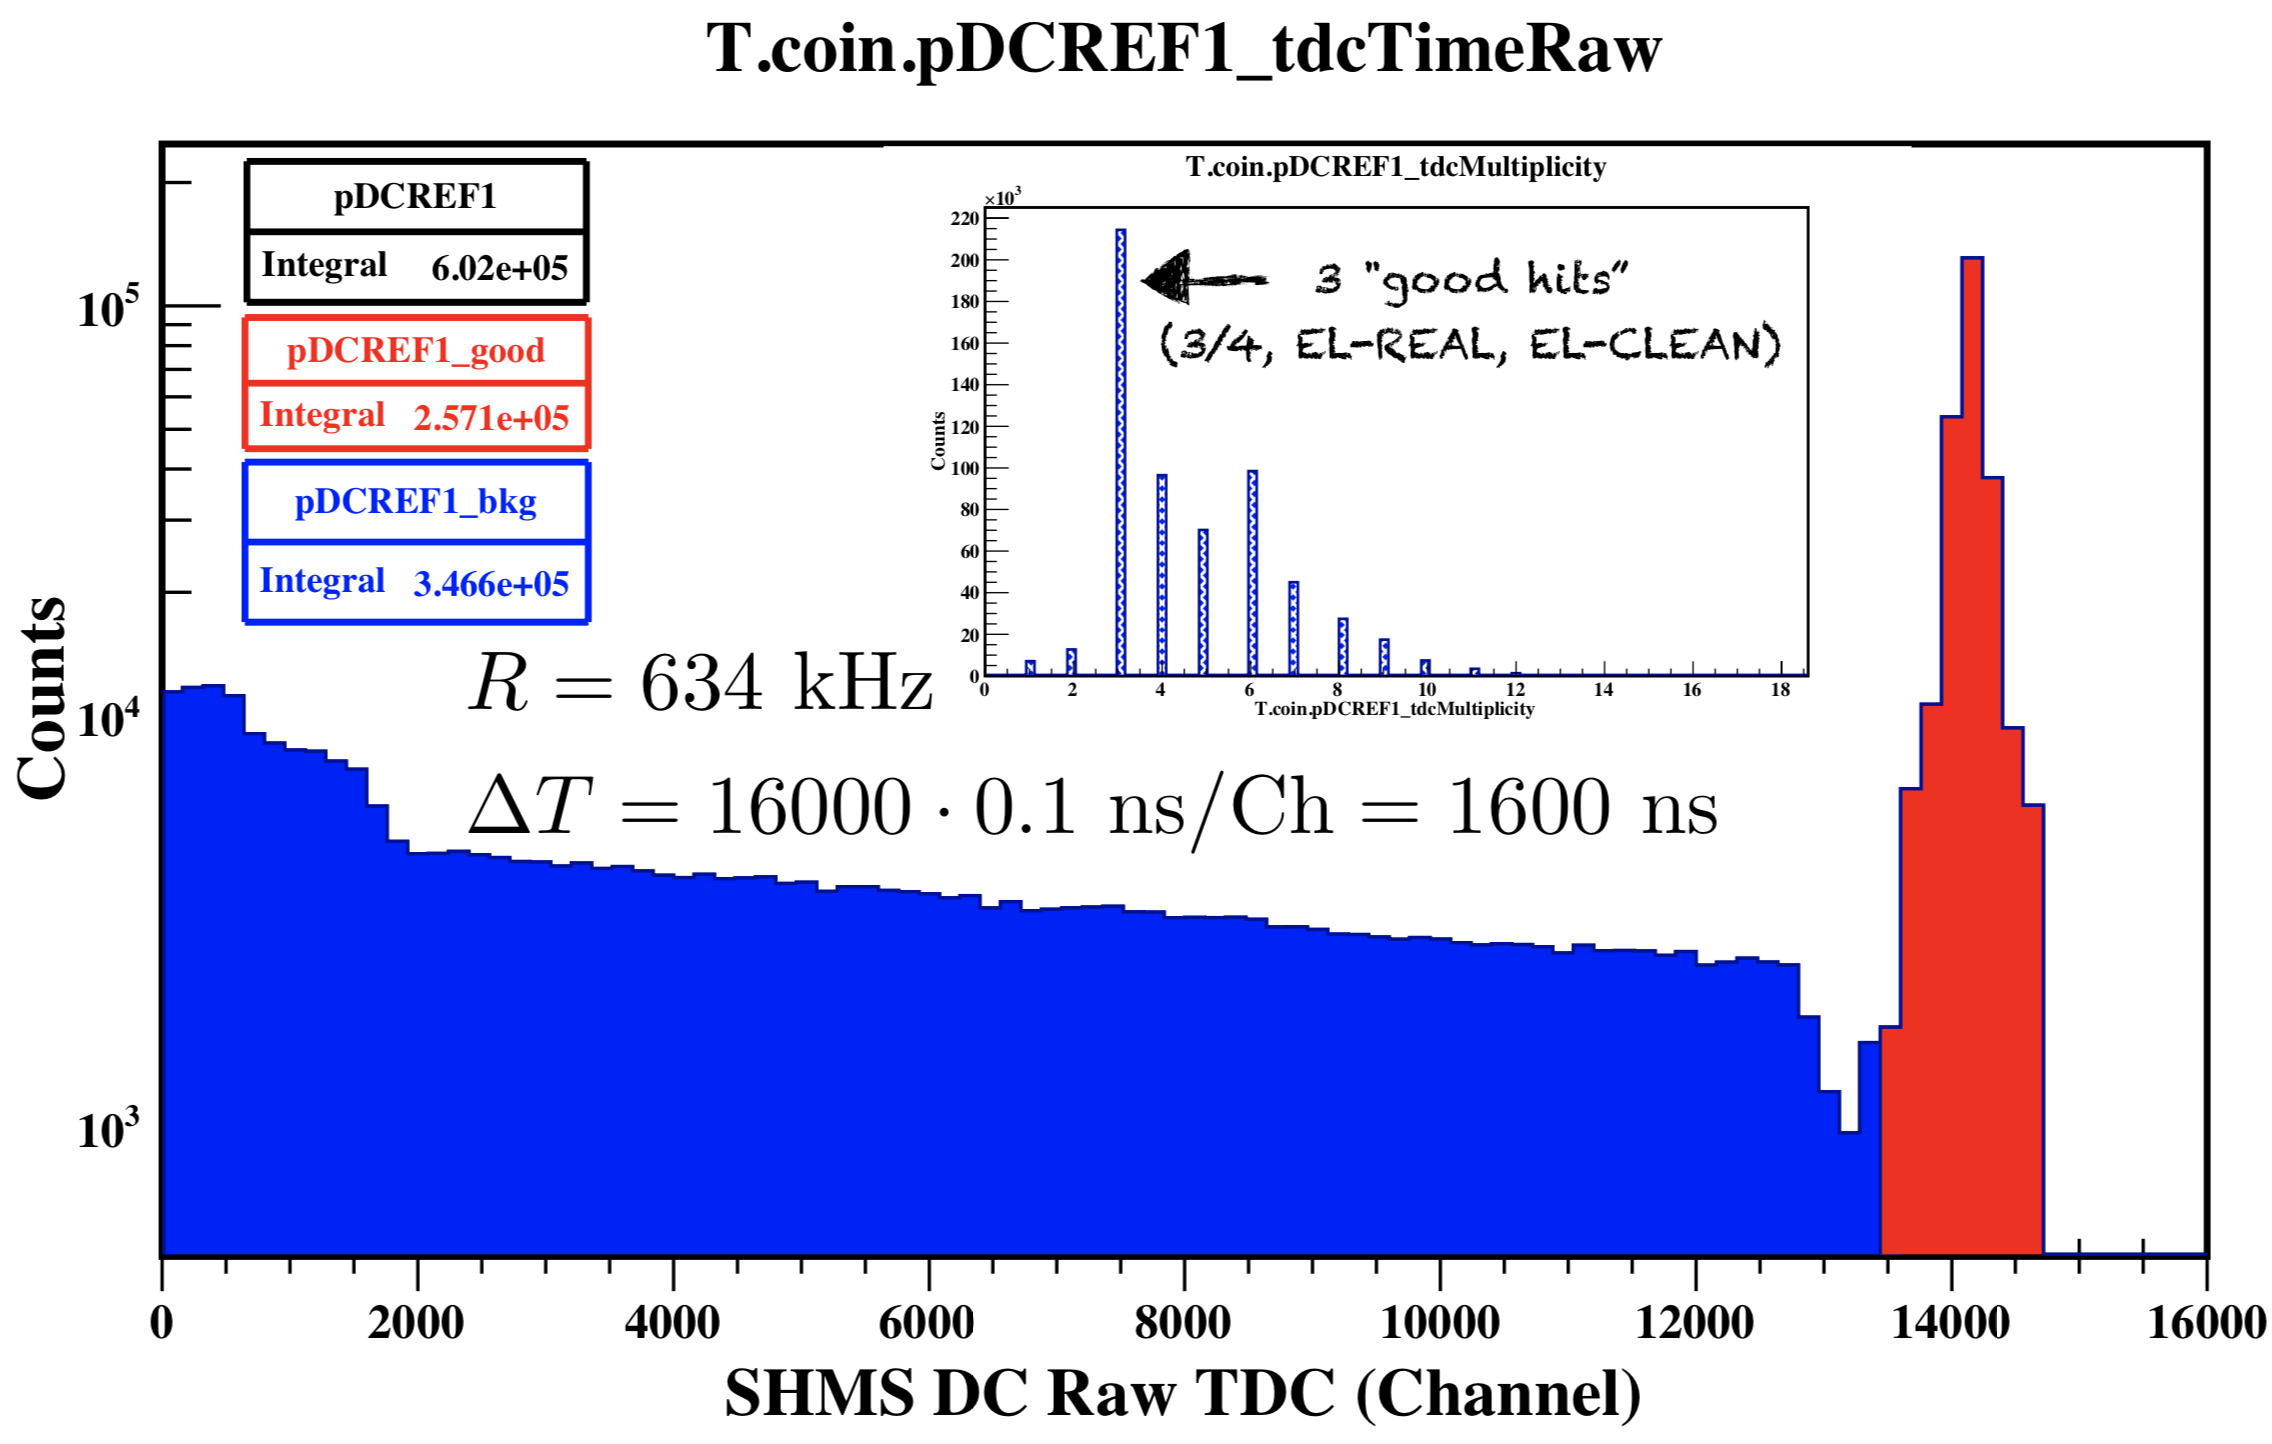
\includegraphics[scale=0.3]{plots/pDCREF_Prob.png}
  \caption{SHMS Reference Time Spectrum for Coincidence Run 3377 of E12-10-003 experiment.}
  \label{fig:pDCref_time_prob}
\end{figure}
Following the poissonian behavior of physics triggers, the probability that 2 hits (\textit{background} and \textit{good hit}) fall within a certain
time window $\Delta T$ at a given physics rate $R$ is given by:
\begin{equation}
  P(\lambda; k) = e^{-\lambda}\frac{\lambda^{k}}{k!}, \text{ where $\lambda=R \Delta T$ and $k=\# \text{ hits}$}
  \label{eq:1}
\end{equation}
From the multiplicity in Figure \ref{fig:pDCref_time_prob}, the reference time had 3 good hits (3/4, EL-REAL, EL-CLEAN, \textcolor{red}{read further}).
For simplicity of the calculation, \textbf{redefine 3 good hits as a single good hit}. Then, from Eq. \ref{eq:1} and Figure \ref{fig:pDCref_time_prob},
the probability of finding 2 hits within the Drift Chamber Time Window is
\begin{align}
  P(\lambda;k) = e^{-R\Delta T}\frac{(R\Delta T)^{2}}{2!} = 0.1865
\end{align}
From Figure \ref{fig:pDCref_time_prob}, this probability is given by taking the ratio of the \textcolor{blue}{background} to the total number of events and divding by
3 to normalize to a single good hit, one obtains
\begin{align}
  P_{data} = \frac{1}{3}\frac{346600}{602000} = 0.1919
\end{align}
The two results agree to $\leq 1\% $. These results indicate that if the reference time had \textbf{NOT} been set for this run, then $\sim 19\%$ of the
events would have the \textbf{WRONG} reference time and a lower tracking efficiency by $\sim 19\%$, hence, \\ \textbf{\textcolor{red}{THE IMPORTANCE OF SETTING THE REFERENCE TIMES!}}
\\ \\
\indent In Hall C, each spectrometer has multiple pre-triggers (3/4, STOF, EL-REAL, EL-CLEAN) which may change depending on the nature of the experiment.
The base pre-trigger is the 3/4, which requires at least 3 of 4 hodoscope planes to fire. During the commissioning phase of the spectrometers, the
reference times was initially defined to be:
\begin{align}
 \text{ref. time} \equiv 3/4 \textit{ \textbf{OR} } \text{STOF} \textit{ \textbf{OR} } \text{EL-REAL} \textit{ \textbf{OR} } \text{EL-CLEAN}
\end{align}
See December 2017 HC-Log Entry \url{https://logbooks.jlab.org/entry/3501198}.  On January 2018, the STOF trigger was removed from this definition,
See HC-Log Entry \url{https://logbooks.jlab.org/entry/3519686}. Finally, on August 2018, EL-CLEAN was removed from the reference time definition, See
HC-Log Entry \url{https://logbooks.jlab.org/entry/3585301}. It was determined that any pre-trigger that require the 3/4 was un-necessary and redundant
to have in the reference time definition, and so they were removed. As of the present day, the reference time definition in Hall C is:
\begin{align}
 \text{ref. time} \equiv 3/4 \textit{ \textbf{OR} } \text{EL-REAL} 
\end{align}
The list of reference time variables is summarized in Tables \ref{tab:Table 1} and \ref{tab:Table 2}.
\begin{table}[h!]
\begin{tabular}{l l l}
Ref. Time Name               & Physical Location & \textit{hcana} Leaf Name  \\
\hline
hFADC\_TREF\_ROC1 & ROC1::SLOT18::Ch11 & \texttt{T.\{spec\}.hFADC\_TREF\_ROC1\_adcPulseTimeRaw}    \\
hTref1            & ROC1::SLOT02::Ch06 & \texttt{T.\{spec\}.hT1\_tdcTimeRaw} \\
hTref2            & ROC1::SLOT20::Ch127 & \texttt{T.\{spec\}.hT2\_tdcTimeRaw} \\
hDCREF1           & ROC3::SLOT08::Ch15 & \texttt{T.\{spec\}.hDCREF1\_tdcTimeRaw} \\
hDCREF2           & ROC3::SLOT16::Ch63 & \texttt{T.\{spec\}.hDCREF2\_tdcTimeRaw} \\
hDCREF3           & ROC3::SLOT04::Ch111 & \texttt{T.\{spec\}.hDCREF3\_tdcTimeRaw} \\
hDCREF4           & ROC3::SLOT13::Ch95 & \texttt{T.\{spec\}.hDCREF4\_tdcTimeRaw} \\
hDCREF5\footnotemark[3]          & ROC3::SLOT02::Ch127 & \texttt{T.\{spec\}.hDCREF5\_tdcTimeRaw} \\

\end{tabular}
\caption{List of HMS Reference Times. Single-Arm DAQ, \textbf{spec=hms}, else if Coincidence Mode DAQ, \textbf{spec=coin}.}
\label{tab:Table 1}
\end{table}
\footnotetext[3]{hDCREF5 reference time signal was added on July 2018. Experiments after this date must also check this reference time.}

\begin{table}[h!]
\begin{tabular}{l l l}
Ref. Time Name               & Physical Location & \textit{hcana} Leaf Name  \\
\hline
pFADC\_TREF\_ROC2 & ROC2::SLOT14::Ch11 & \texttt{T.\{spec\}.pFADC\_TREF\_ROC2\_adcPulseTimeRaw}    \\
pTref1            & ROC2::SLOT20::Ch15 & \texttt{T.\{spec\}.pT1\_tdcTimeRaw} \\
pTref2            & ROC2::SLOT19::Ch31 & \texttt{T.\{spec\}.pT2\_tdcTimeRaw} \\
pDCREF1           & ROC6::SLOT06::Ch79 & \texttt{T.\{spec\}.pDCREF1\_tdcTimeRaw} \\
pDCREF2           & ROC6::SLOT07::Ch79 & \texttt{T.\{spec\}.pDCREF2\_tdcTimeRaw} \\
pDCREF3           & ROC6::SLOT08::Ch79 & \texttt{T.\{spec\}.pDCREF3\_tdcTimeRaw} \\
pDCREF4           & ROC6::SLOT09::Ch79 & \texttt{T.\{spec\}.pDCREF4\_tdcTimeRaw} \\
pDCREF5           & ROC6::SLOT10::Ch79 & \texttt{T.\{spec\}.pDCREF5\_tdcTimeRaw} \\
pDCREF6           & ROC6::SLOT11::Ch47 & \texttt{T.\{spec\}.pDCREF6\_tdcTimeRaw} \\
pDCREF7           & ROC6::SLOT12::Ch47 & \texttt{T.\{spec\}.pDCREF7\_tdcTimeRaw} \\
pDCREF8           & ROC6::SLOT13::Ch47 & \texttt{T.\{spec\}.pDCREF8\_tdcTimeRaw} \\
pDCREF9           & ROC6::SLOT14::Ch15 & \texttt{T.\{spec\}.pDCREF9\_tdcTimeRaw} \\
pDCREF10          & ROC6::SLOT15::Ch47 & \texttt{T.\{spec\}.pDCREF10\_tdcTimeRaw} \\

\end{tabular}
\caption{List of SHMS Reference Times. Single-Arm DAQ, \textbf{spec=shms}, else if Coincidence Mode DAQ, \textbf{spec=coin}.}
\label{tab:Table 2}
\end{table}

\newpage

Associated with each physical detector and pseudo-detector \texttt{(TRIG)}, are specific reference times from the Tables \ref{tab:Table 1} and \ref{tab:Table 2}.
The reference times associated with each detector are summarized below.


\begin{table}[h!]
\begin{tabular}{l l l}
SPEC  & DETEC & Ref. Time Name  \\
\hline
HMS & AERO[adc] & hFADC\_TREF\_ROC1 \\
& CAL[adc] & hFADC\_TREF\_ROC1 \\
& CER[adc] & hFADC\_TREF\_ROC1 \\
& DC[tdc] & hDCREF1, hDCREF5 \\
& HODO[adc] & hFADC\_TREF\_ROC1 \\
& HODO[tdc] & hTref2 \\
& TRIG[adc] &  hFADC\_TREF\_ROC1 \\
& TRIG[tdc] & hTref1 \\
\\
SHMS & AERO[adc] & pFADC\_TREF\_ROC2 \\
& CAL[adc] & pFADC\_TREF\_ROC2 \\
& HGCER[adc] & pFADC\_TREF\_ROC2 \\
& NGCER[adc] & pFADC\_TREF\_ROC2 \\
& DC[tdc] & pDCREF 1-10 \\
& HODO[adc] & pFADC\_TREF\_ROC2 \\
& HODO[tdc] & pTref1, pTRef2 \\
& TRIG[adc] & pFADC\_TREF\_ROC2 \\
& TRIG[tdc] & pTref2 \\
\end{tabular}
\caption{List of Detector Reference Times, which applies for both Singles and Coin DAQ modes. The table shows which reference times are being subtracted from each
detector or pseudo-detector signal.}
\label{tab:Table 3}
\end{table}
\noindent From the summary Table \ref{tab:Table 3} above, it is important to note that the all detectors in HMS / SHMS use the same ADC reference time signal in their respective spectrometers (indicating all ROCs FADCs appear to be synchronized),
however, with respect to the TDCs, each TDC receives a distinct copy of the reference times with the exception of the Drift Chambers in ROC3, as this crate has the capability to synchronize all TDCs it holds. \\
\\
\noindent To determine what values to set the reference time cuts, it is recommended that a multiplicity cut be made on the variable being looked at. The
multiplicity of a given variable refers to the total number of adc or tdc hits per event. If the event was a true physics event, most likely the
total number of reference time hits will be one. If the reference time was OR'ed from \textit{n} pre-triggers, and the pre-triggers are assumed to be
almost 100\% efficient, then a true physics event will most likely have \textit{n} hits. In this case, it is recommended that a multiplicity cut requiring
\textit{n} hits be made in order to clean the reference time spectrum and better select a reference time cut value. It is easier to look a the multiplicity
leaf variable itself, and determine which multiplicity cut to make.
\begin{figure}[H]
  \captionsetup{justification=raggedright,singlelinecheck=false}
  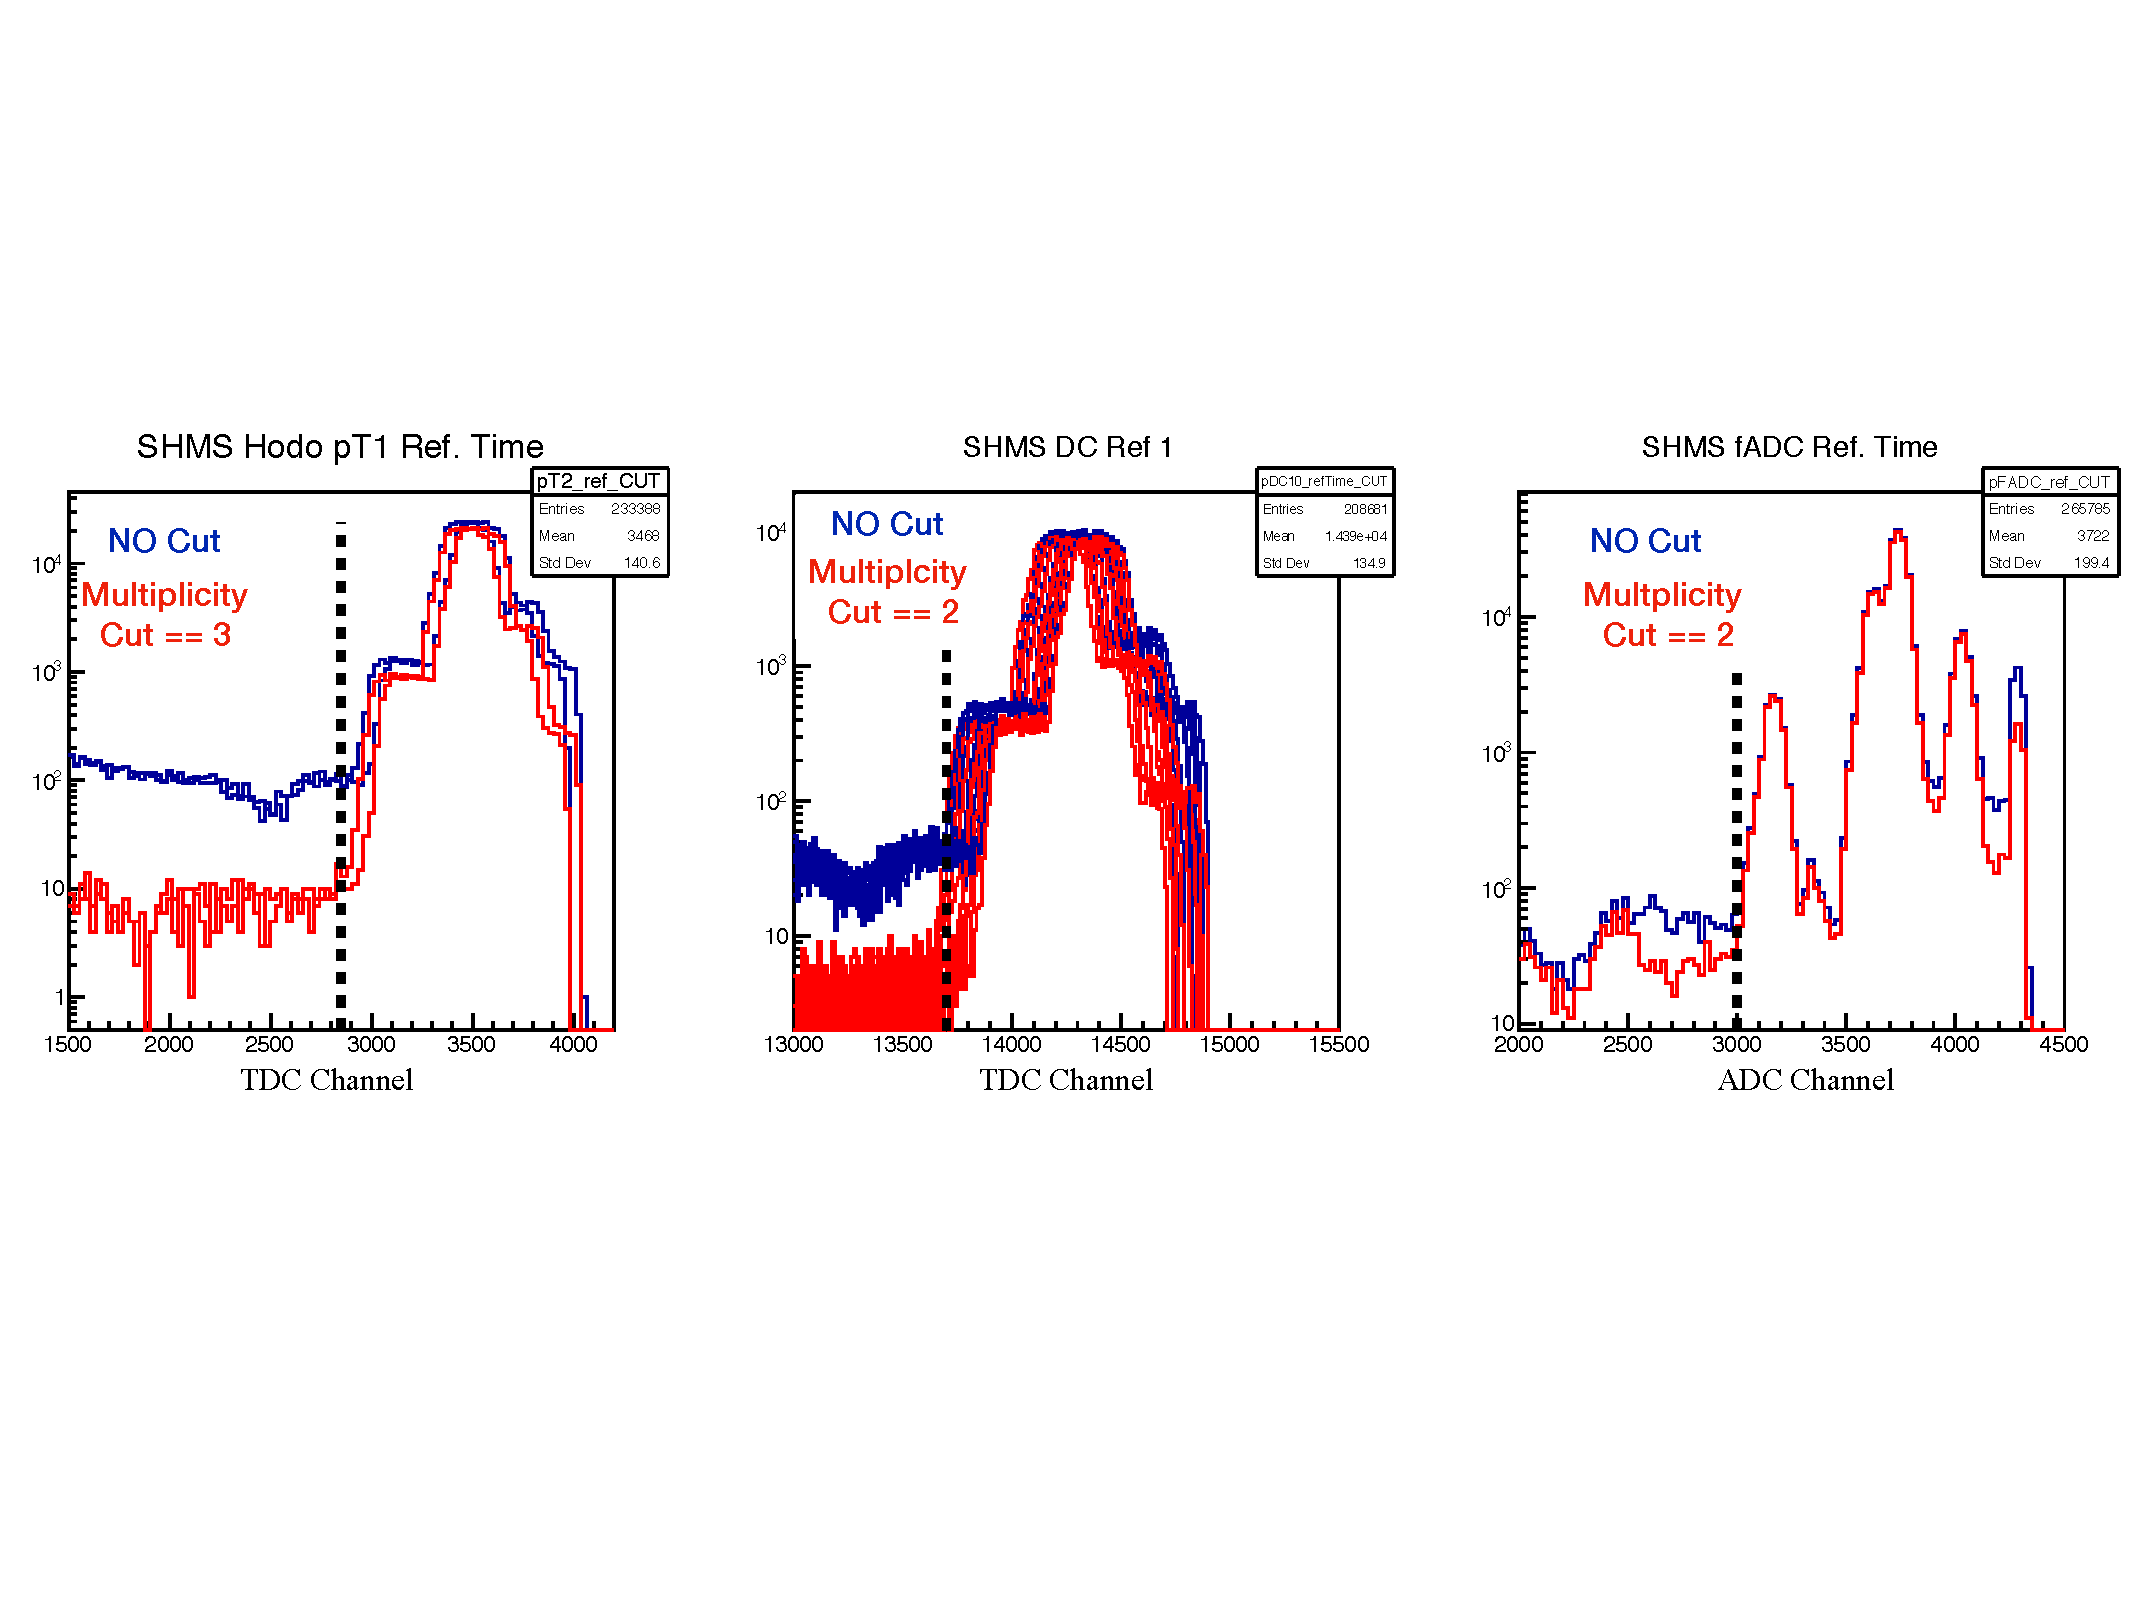
\includegraphics[scale=0.5]{plots/shms_ref_times.pdf}
  \caption{SHMS Reference Time Cuts for Coincidence Run 3289 of E12-10-003 experiment. The conversion from TDC Channel to time is $\sim$ 0.1 ns/Ch. The conversion from ADC Channel to time is 0.0625 ns/Ch. }
  \label{fig:shms_ref_times}
\end{figure}
Figure \ref{fig:shms_ref_times} shows the reference times used in the analysis. The
multiplicity cut reduces the background, although not completely so a judgement of where to place the cut has to be made. The shapes of the reference times may change
depending on the experiment trigger used. To the left of the cut, are the reference times from various sources of background. 
Once the reference time cut has been determined, the corresponding parameter files must be updated with the cut values. The parameter files to be modified are
located at: 
\begin{flushleft}
  \texttt{hallc\_replay/PARAM/HMS/GEN/h\_reftime\_cut.param} \\
  \texttt{hallc\_replay/PARAM/SHMS/GEN/p\_reftime\_cut.param} \\
  \texttt{hallc\_replay/PARAM/TRIG/t[daq\_mode].param\footnote{If the experiment uses the DAQ in single arm mode (separate HMS/SHMS CODA GUI), the \texttt{TRIG} parameter file
    modified must be \texttt{thms.param} or \texttt{tshms.param}},  [daq\_mode]=hms, shms, coin} 
\end{flushleft}
and the parameter files look as follows:
\begin{figure}[H]
  \captionsetup{justification=raggedright,singlelinecheck=false}
\begin{center}
  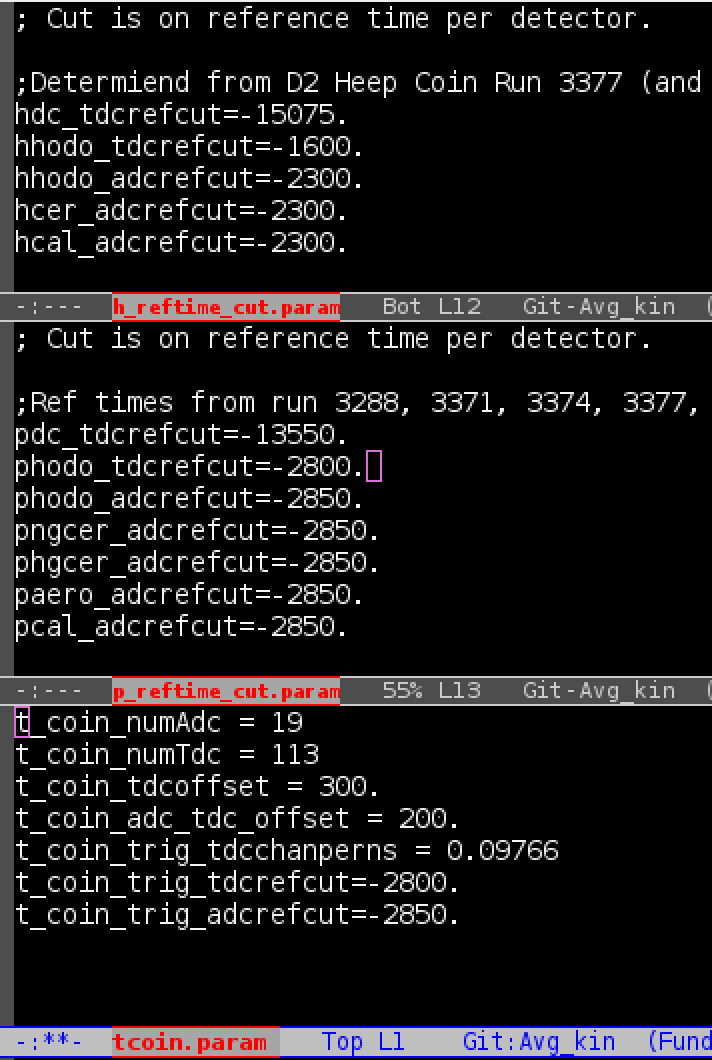
\includegraphics[scale=0.5]{plots/reftime_parm.png}
\end{center}
\caption{HMS (top), SHMS (middle), COIN TRIG[bottom] reference time parameter files. The set cut values have a negative sign as opposed to the histograms in Figure \ref{fig:shms_ref_times}.
  The ADC ref. time is common to the Calorimeter, Cherenkovs and Hodoscopes.}
  \label{fig:reftime_parm}
\end{figure}
\noindent Once the reference time parameter file has been updated, the the data must be replayed so that the correct reference time is selected before moving to the
next step in the analysis procedure. In principle, the reference time should be relatively stable, but it is worth checking for different kinematics as well as different
trigger configurations. It is recommended that for each kinematic setting a single (or combined) run with enough statistics ($\sim$ 1 M events) is selected to set (or check) the
reference time cuts.
\section{\textbf{Set Detector Time Window Cuts}}
The next step in the analysis procedure is setting up the detector time window cuts. These are necessary to reduce sources of background that slips into the detector
time windows when detecting the physics signals of interest. The time window cut is made on a time difference between the ADC and TDC times on a PMT basis  for all the detectors
except the Drift Chamber, which cut on the raw drift times for each plane.  The time difference is defined in \textit{hcana} as
\begin{align}
  &\texttt{AdcTdcDiffTime} = \texttt{TdcTime[ipmt] - AdcPulseTime[ipmt]} \text{ HODO} \\
  &\texttt{AdcTdcDiffTime} = \texttt{HodoStartTime - AdcPulseTime[ipmt]} \text{ CER, HGCER, NGCER, CAL, AERO}
\end{align}
where the \texttt{HodoStartTime} is the Hodoscope time projected at the focal plane, and the \texttt{TdcTime, AdcPulseTime} is the detector (TDC,ADC) pulse time for a given PMT in that detector.
If the event is truly a physics event originating from the target, then in principle, the time difference should be a $\delta$-function, however due to the finite
detector resolutions, it has a finite width and gaussian in shape. Events that are far away from the main peak are clearly out-of-time indicating that the ADC pulse time and
TDC Time are NOT correlated with the same event, and a time window cut must be made. With respect to the Drift Chambers, a cut on the raw drift time spectrum to reduce the background
from multiple hits. Similarly to the reference time cuts, the detector time window cuts are set via a parameter cut file associated with the detector.
The detector variable names used as well as the parameter files used to set the cuts are summarized below.
\begin{table}[h!]
  \small
\begin{tabular}{l l l}
\textbf{Detector} & \textit{hcana} \textbf{Leaf Name} & \textbf{Place-Holders} \\
\hline
Hodoscopoes &  \texttt{H.hod.[pl].Good[side]AdcTdcDiffTime[ipmt]} & \texttt{[pl]:1x|1y|2x|2y [side]:Pos|Neg} \\
& \texttt{H.hod.[pl].Good[side]AdcMult[ipmt]} & \\ \\
Calorimeter &  \texttt{H.cal.[pl].good[side]AdcTdcDiffTime[ipmt]} & \texttt{[pl]:1pr|2ta|3ta|4ta [side]:Pos|Neg} \\
& \texttt{H.cal.[pl].good[side]AdcMult[ipmt]} & \\ \\
Cherenkov   &  \texttt{H.cer.goodAdcTdcDiffTime[ipmt]} & \\
& \texttt{H.cer.goodAdcMult[ipmt]} & \\ \\
Drift Chamber & \texttt{H.dc.[pl].rawtdc} & \texttt{[pl]:1u1|1u2|...2x2|2v1|...} \\
& \texttt{H.dc.[pl].nhit} &
\end{tabular}
\caption{HMS detectors variable names are summarized. The \texttt{[impt]} index emphasizes the leaf variables are arrays whose indices are the PMTs, but do NOT
form part of the leaf name. }
\label{tab:Table 4}
\end{table}
\begin{table}[h!]
  \small
\begin{tabular}{l l l}
\textbf{Detector} & \textit{hcana} \textbf{Leaf Name} & \textbf{Place-Holders} \\
\hline
Hodoscopoes &  \texttt{P.hod.[pl].Good[side]AdcTdcDiffTime[ipmt]} & \texttt{[pl]:1x|1y|2x|2y [side]:Pos|Neg} \\
& \texttt{P.hod.[pl].Good[side]AdcMult[ipmt]} & \\ \\
Pre-Shower & \texttt{P.cal.pr.good[side]AdcTdcDiffTime} & \texttt{[side]:Pos|Neg} \\
& \texttt{P.cal.pr.good[side]AdcMult[ipmt]} & \\ \\
Calorimeter &  \texttt{P.cal.fly.goodAdcTdcDiffTime[ipmt]} &  \\
& \texttt{P.cal.fly.goodAdcMult[ipmt]} & \\ \\
Cherenkov   &  \texttt{P.[det].goodAdcTdcDiffTime[ipmt]} & \texttt{[det]:hgcer|ngcer} \\
& \texttt{P.[det].goodAdcMult[ipmt]} & \\ \\
Drift Chamber & \texttt{P.dc.[pl].rawtdc} & \texttt{[pl]:1u1|1u2|...2x2|2v1|...} \\
& \texttt{P.dc.[pl].nhit} & 
\end{tabular}
\caption{SHMS detectors variable names are summarized. The \texttt{[impt]} index emphasizes the leaf variables are arrays whose indices are the PMTs, but do NOT
form part of the leaf name. }
\label{tab:Table 5}
\end{table} 
\begin{table}[h!]
\begin{tabular}{l l l}
\textbf{Detector} & \textit{hcana} \textbf{Leaf Name} & \textbf{Place-Holders} \\
\hline
TRIG & \texttt{T.[spec].*} & \texttt{[spec]: hms | shms | coin} \\
\end{tabular}
\caption{Trigger detector variable names are summarized. The \texttt{[spec]} refers to the DAQ mode. If single-arm mode or coincidence mode. NOTE: singles in
coincidence mode DAQ is considered \texttt{coin}.}
\label{tab: Table 6}
\end{table} 
\begin{figure}[H]
  \captionsetup{justification=raggedright,singlelinecheck=false}
  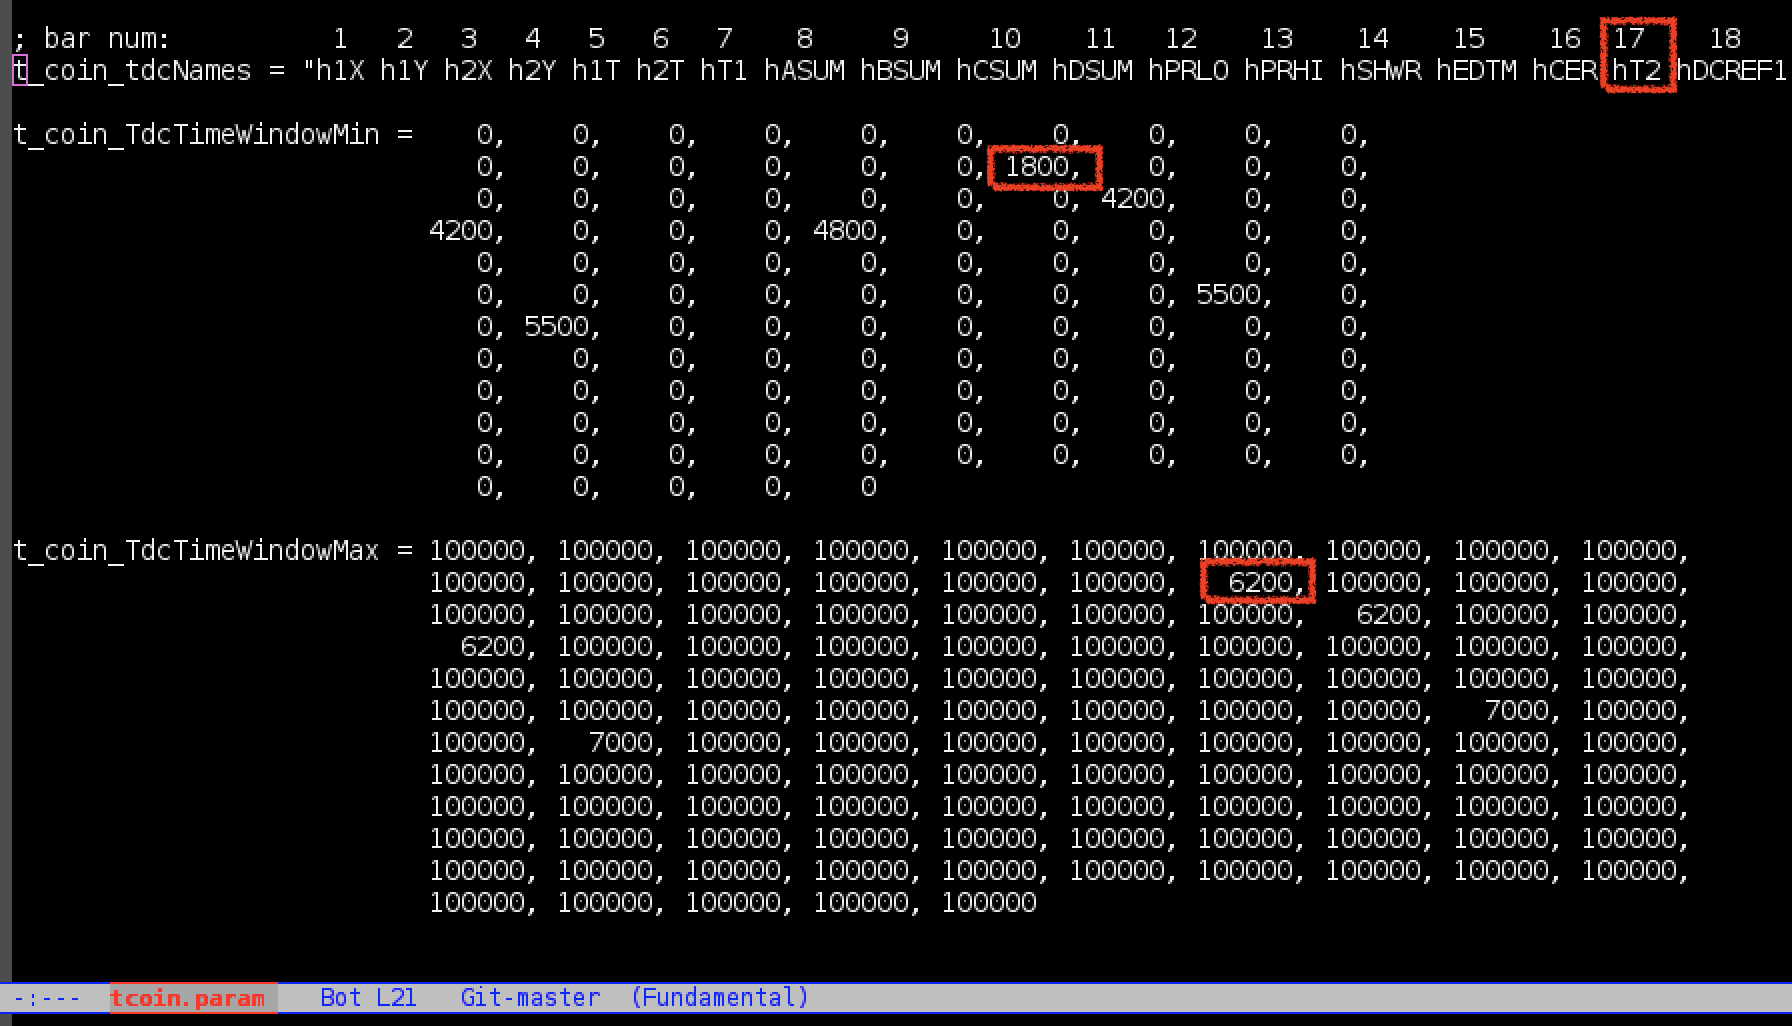
\includegraphics[scale=0.3]{plots/tcoin_parm.png}
  \caption{\texttt{TRIG} Detector parameter file for coincidence mode DAQ. The \textcolor{red}{rectangles} highlight a variable of interest (hT2), and the Min/Max
  Time Window Cut for that variable, indexed at 17.}
  \label{fig:tcoin_parm}
\end{figure}
\noindent Setting the \texttt{TRIG} pseudo-detector Time Window cuts is \textbf{NOT} as obvious as a normal detector. First, the variables from the \texttt{TRIG} that
will be used in the analysis need to be determined. Then, the index corresponding to the variables of interest need to be determined from the \texttt{TRIG} parameter file.
Finally, once the Time Window cut values have been determined, they need to be updated in the parameter file. See Figure \ref{fig:tcoin_parm} for reference.
\\

\indent Similarly to the reference time histograms, it might be useful to put a multiplicity cut on the detector time variables in Tables \ref{tab:Table 4}, \ref{tab:Table 5} and
\ref{tab: Table 6}. An important point to make is the variables with \texttt{nhit} in their name. This represents the maximum number of hits per event, and so when filling
the raw tdc time in the Drift Chambers, this histogram must be filled by looping over all possible \texttt{nhit} hits per event entry. Some examples of the detector time
difference and raw time histograms are shown below.
\begin{figure}[H]
  \captionsetup{justification=raggedright,singlelinecheck=false}
  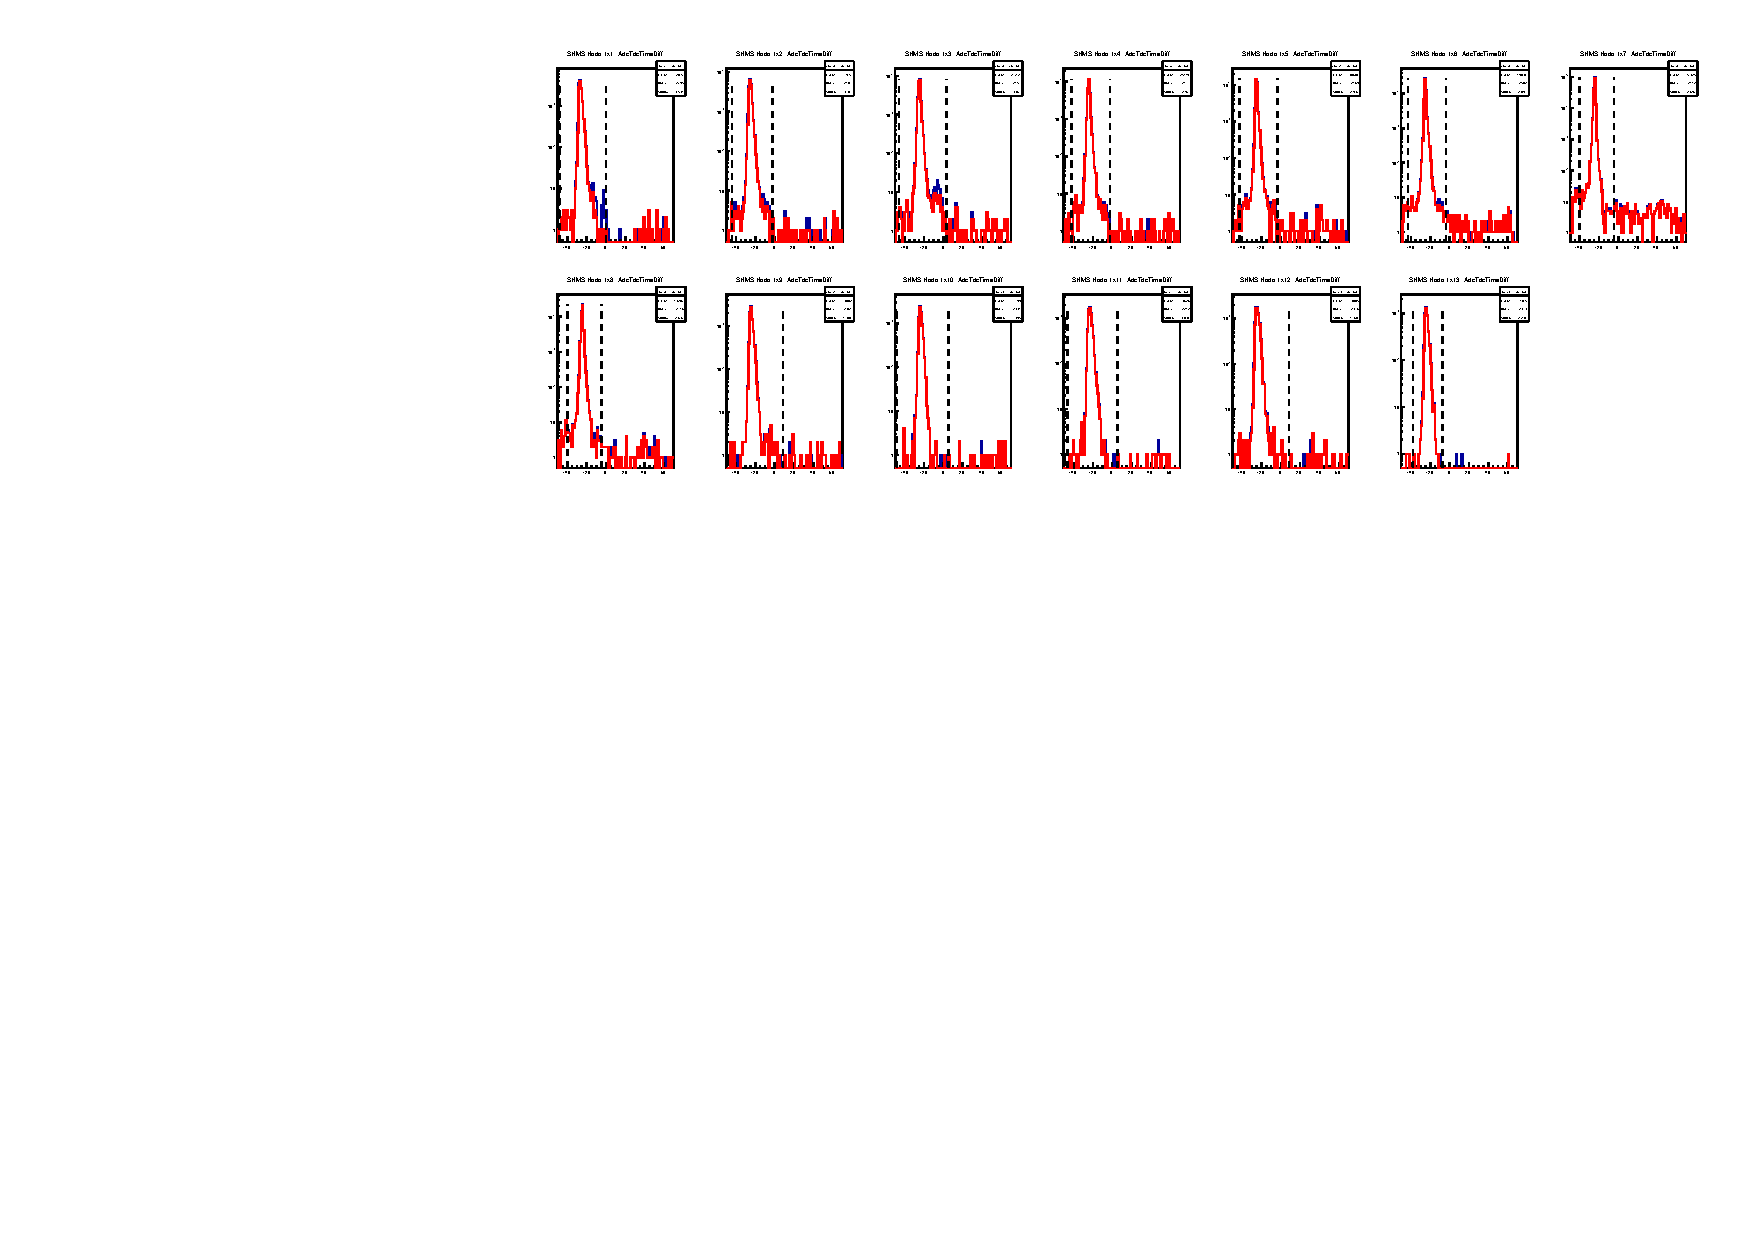
\includegraphics[scale=0.95]{plots/pHodo_1xGoodNeg.pdf}
  \caption{SHMS Hodoscope 1X Neg Time Difference. Coincidence Run 3289 of E12-10-003 experiment.}
  \label{fig:shms_hodo_difftime}
\end{figure}
\begin{figure}[H]
  \captionsetup{justification=raggedright,singlelinecheck=false}
  \includegraphics[scale=0.95]{plots/pCal_Row9.pdf}
  \caption{SHMS Calorimeter Row9 Channels Time Difference. Coincidence Run 3289 of E12-10-003 experiment.}
  \label{fig:shms_cal_difftime}
\end{figure}
\begin{figure}[H]
  \captionsetup{justification=raggedright,singlelinecheck=false}
  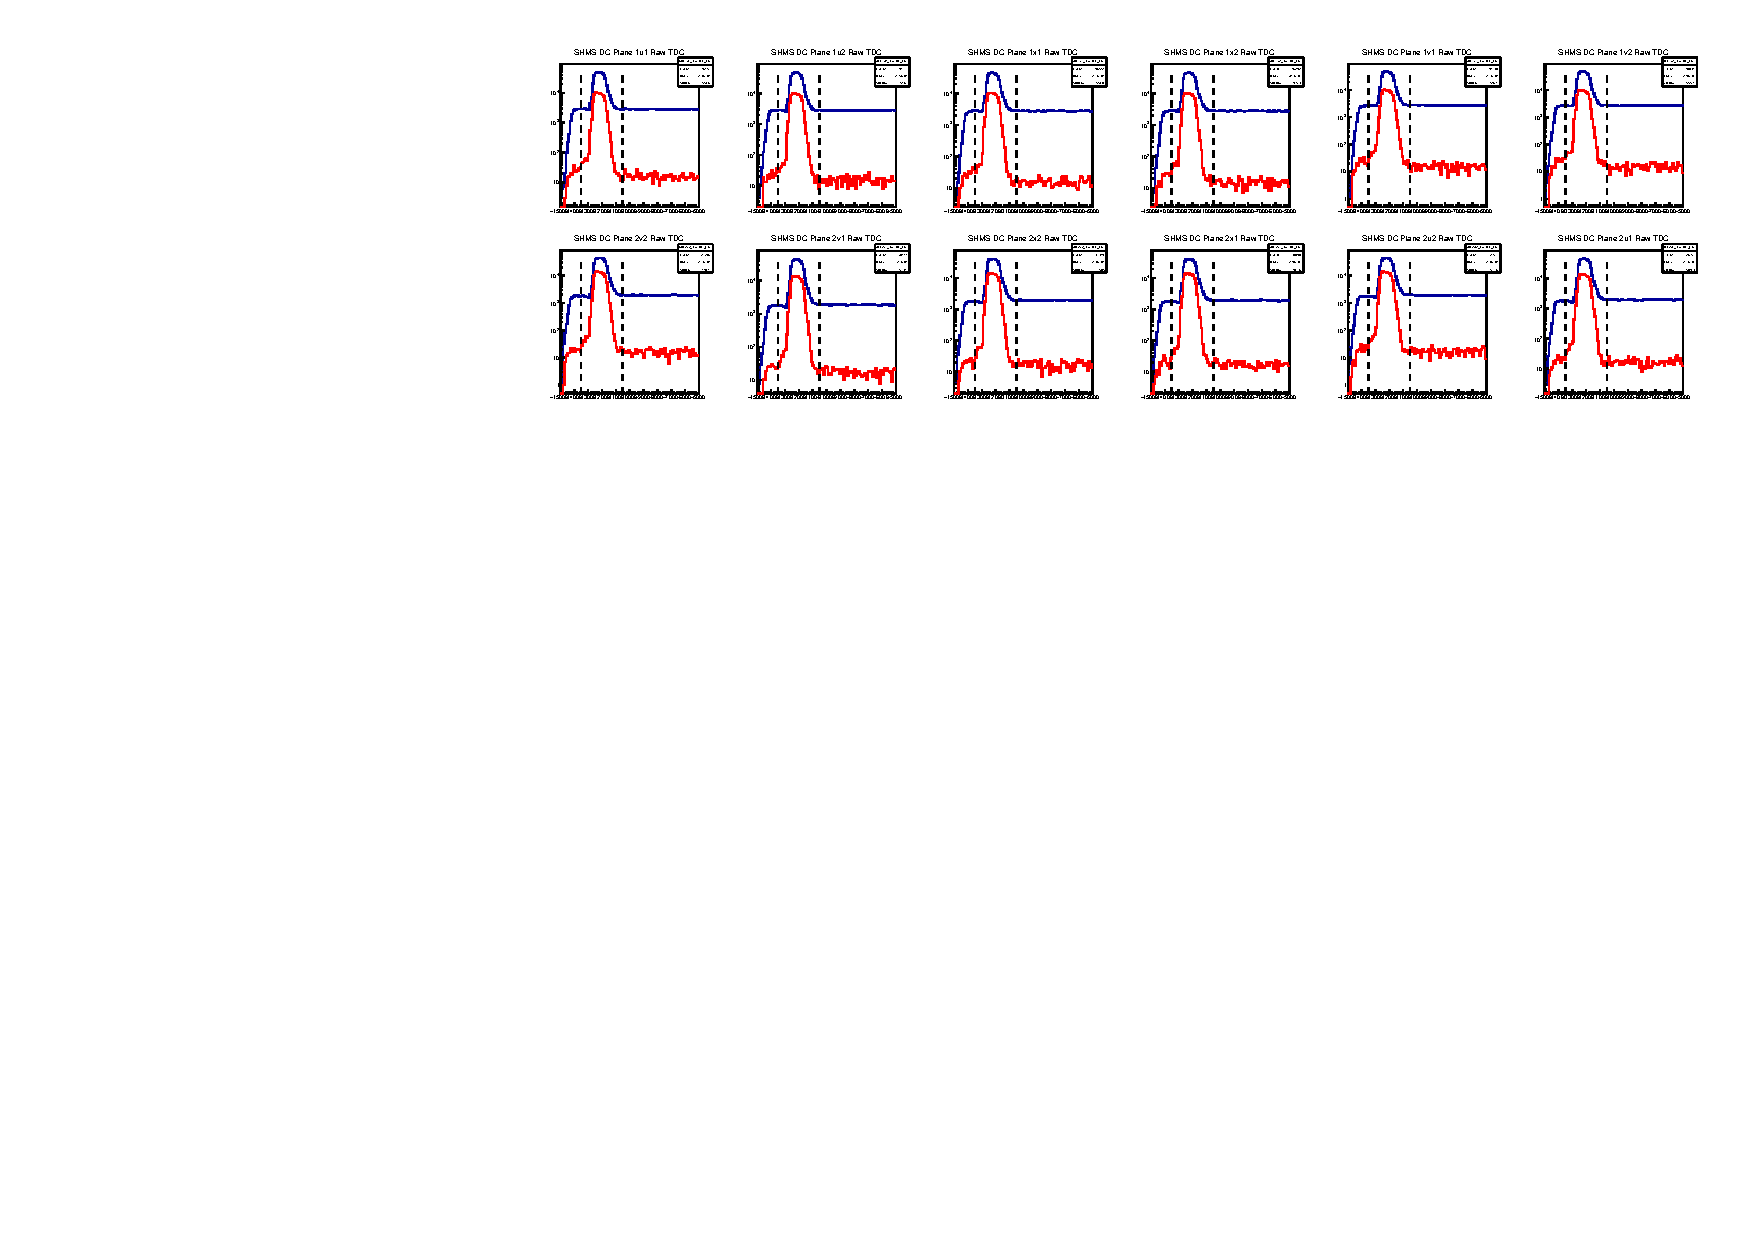
\includegraphics[scale=0.95]{plots/pDC_rawTDC_window.pdf}
  \caption{SHMS Drift Cambers Raw TDC Time. Coincidence Run 3289 of E12-10-003 experiment.}
  \label{fig:shms_dc_rawtime}
\end{figure}
\begin{figure}[H]
  \begin{center}
  \captionsetup{justification=raggedright,singlelinecheck=false}
  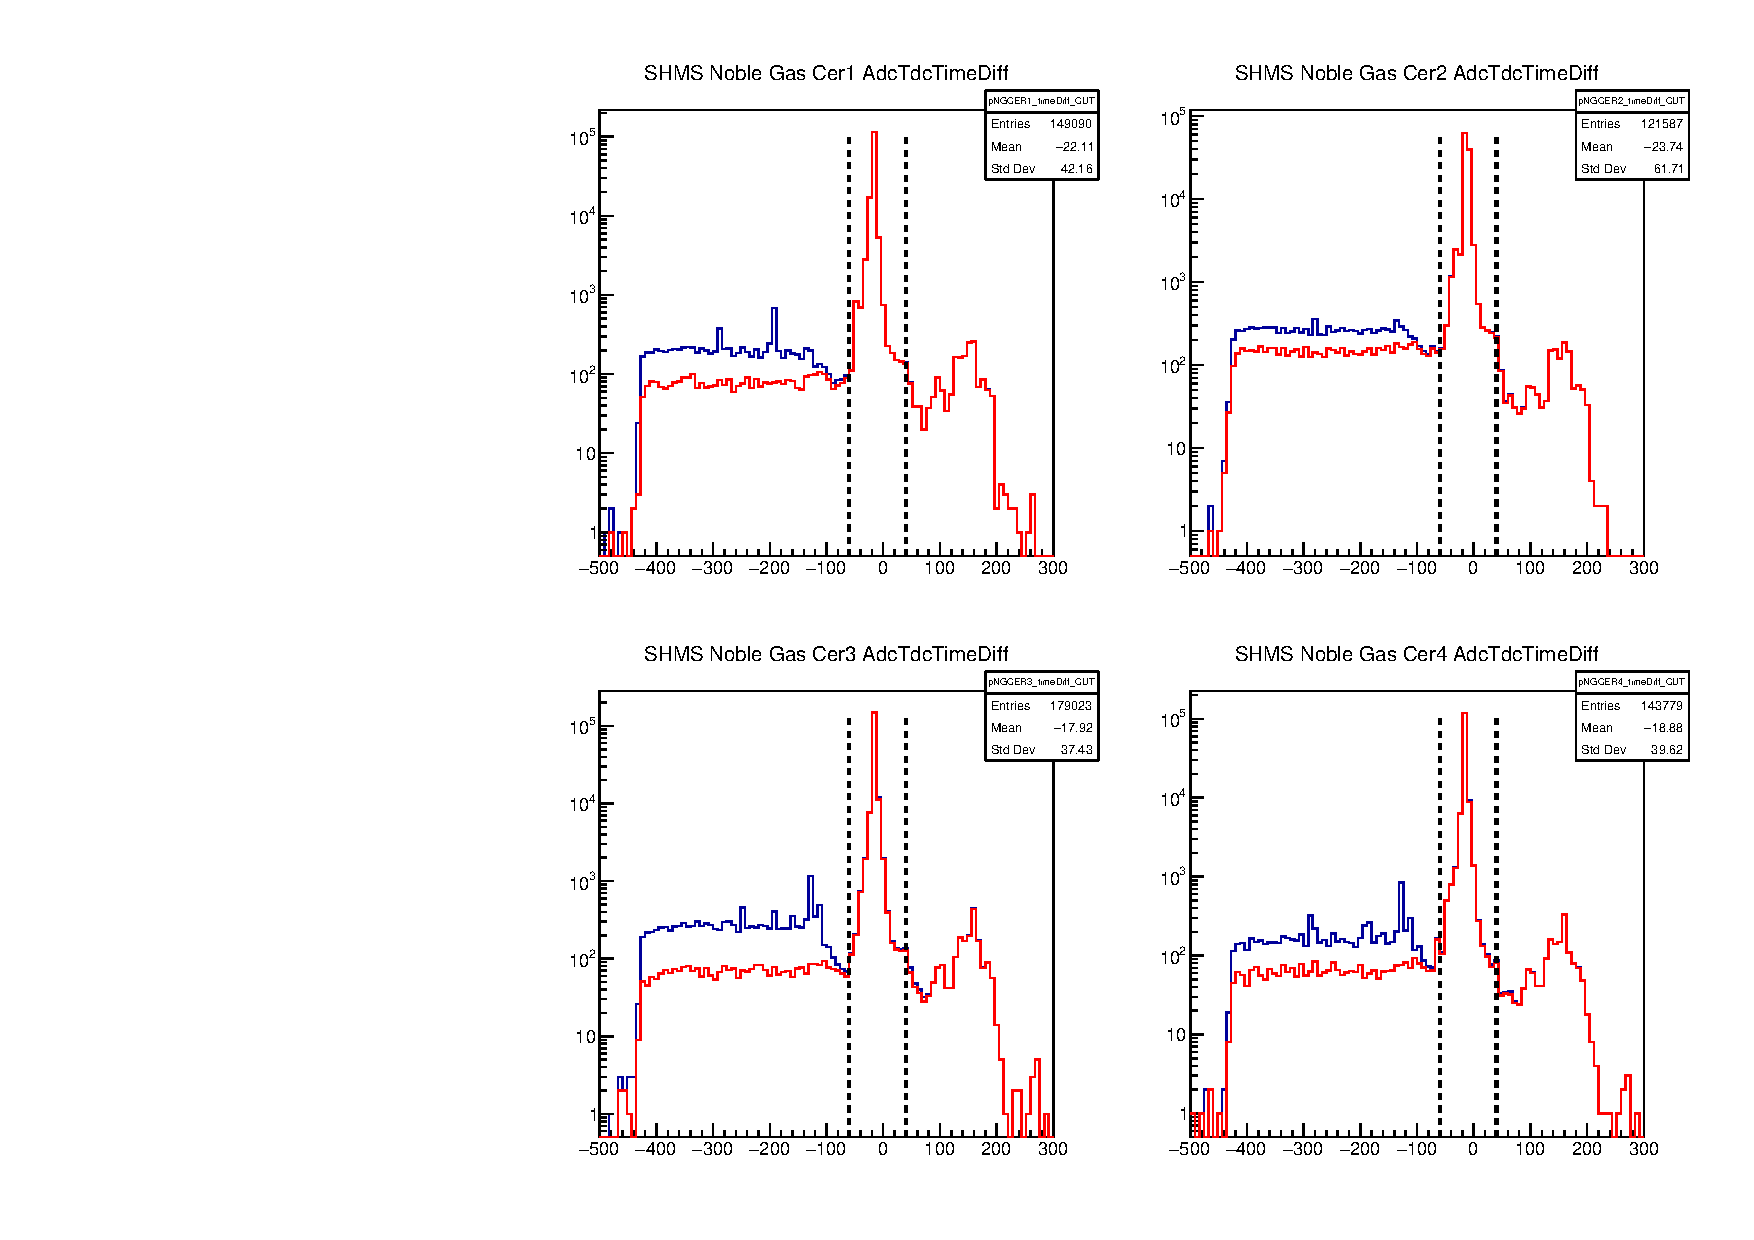
\includegraphics[scale=0.4]{plots/pNGCER_timeWindow.pdf}
  \caption{SHMS Noble Gas Cherenkov Time Difference. Coincidence Run 3289 of E12-10-003 experiment.}
  \label{fig:shms_ngcer_difftime}
  \end{center}
\end{figure}

\noindent From the plots shown above, the \textcolor{red}{red histograms}, have a multplicity cut, and the \textcolor{blue}{blue histograms} have no multiplicity cut. A main
peak is clearly distiguishable in all plots. 
Once the detector time window cuts have been determined, they are set in the detector cuts parameter files located at:
\begin{flushleft}
  \texttt{hallc\_replay/PARAM/HMS/\{DETEC\}/h\{detec\}\_cuts.param} \\
  \texttt{hallc\_replay/PARAM/SHMS/\{DETEC\}/p\{detec\}\_cuts.param} \\
  \texttt{hallc\_replay/PARAM/TRIG/t\{spec\}.param} 
\end{flushleft}
where \texttt{DETEC(HMS): CAL, CER, DC, HODO, AERO}, \texttt{DETEC(SHMS): CAL, HGCER, NGCER, DC, HODO, AERO}, and
\texttt{spec: hms, shms, coin}.
For the aerogel, no examples were shown, but in principle, in terms of setting the time window cuts should be similar procedure.
For examples of how the parameter file to be modified looks like for all the detectors, see Appendix \ref{appendix:AppxA}.
\section{Detector Calibrations}
After selecting the right reference times and setting proper detector time window cuts, detector calibrations can be started. Ideally, one would
use specific runs for calibrations in which most of the focal plane is illuminated. Sometimes, a magnet de-focused run is used, however, one has to be
careful as some calibrations actually depend on the reconstructed quantities at the target (Calorimeter), and hence knowledge of the reconstruction
spectrometer optics. In this case, it is recommended to use single-arm runs over coincidence runs, as the latter will be more constrained. In this section,
I will point to more detailed documentation on the Hall C Document Database (DocDB), as well as the document with the instructions to run the calibration.

\subsection{Hodoscopes}
The hodoscopoes Calibration code and README files with the instructions on how to do the calibration is found on:
\begin{center}
  \url{https://github.com/JeffersonLab/hallc_replay/tree/master/CALIBRATION/hms_hodo_calib} \\
   \url{ https://github.com/JeffersonLab/hallc_replay/tree/master/CALIBRATION/shms_hodo_calib}
\end{center}

Additional documentation on the Hodoscope calibration can be found on the Hall C Document DataBase:
\begin{center}
  \url{https://hallcweb.jlab.org/DocDB/0009/000970/001/hodo_calib.pdf}
\end{center}

\subsection{Drift Chambers}
The Drift Chambers Calibration code and README files with the instructions on how to do the calibration is found on:
\begin{center}
\url{https://github.com/JeffersonLab/hallc_replay/tree/master/CALIBRATION/dc_calib/scripts}  
\end{center}

Additional documentation on the Drift Chamber calibration can be found on the Hall C Document DataBase:
\begin{center}
  \url{https://hallcweb.jlab.org/DocDB/0008/000863/003/HallC-Software-Workshop_pdf.pdf}\\
  \url{https://hallcweb.jlab.org/DocDB/0008/000842/003/report.pdf}
\end{center}
\subsection{Calorimeters}
The Calorimeter Calibration code and README (howto.txt) files with the instructions on how to do the calibration is found on:
\begin{center}
  \url{https://github.com/JeffersonLab/hallc_replay/tree/master/CALIBRATION/hms_cal_calib} \\
  \url{https://github.com/JeffersonLab/hallc_replay/tree/master/CALIBRATION/shms_cal_calib}
\end{center}

Additional documentation on the Calorimeter can be found on the Hall C Document DataBase:
\begin{center}
\url{https://hallcweb.jlab.org/DocDB/0008/000809/001/NIMarticleOverview.pdf}
\end{center}
\subsection{Cherenkovs}
The Cherenkovs Calibration code and README files with instructions on how to do the calibration is found on:
\begin{center}
  \url{https://github.com/JeffersonLab/hallc_replay/tree/master/CALIBRATION/hms_cer_calib} \\
  \url{https://github.com/JeffersonLab/hallc_replay/tree/master/CALIBRATION/shms_hgcer_calib}
\end{center}
Additional documentation on the Cherenkovs can be found on the Hall C Document DataBase:
\begin{center}
\url{https://hallcweb.jlab.org/DocDB/0008/000893/001/HGC_Calibration.pdf}
\end{center}
\section{Summary of Analysis Procedure}
\textbf{STEP 1:} Set the reference time cut parameters, as they are needed to select the correct pre-trigger correlated with each event (see Section \ref{sec:ref_time_cuts}).
\begin{itemize}
\item You can select a representative run for each kinematic setting of the experiment to check and set the reference time cut parameters. Check if the reference time histograms per
  kinematic setting shift significantly, in which case, you may need to set the reference time parameters per setting.  
\item After the reference time parameters have been set, make sure to replay the data before moving on to the next step (detector time windows) to ensure
  that the correct reference times (determined by the reference time parameter file in step 1) are selected per event. 
\end{itemize}
\textbf{STEP 2:} Set the detector time window cut parameters, as they are needed to reduce sources of background that slips into the detector readout windows when detecting the physics signals of interest.
\begin{itemize}
  \item Similarly to step 1, you can select a representative run for each kinematic setting of the experiment to check whether the relevant histograms shift per setting, in which case the detectors time window cuts
    may need to be determined for each setting.
  \item After the detector time window cut parameters have been set, make sure to replay the data before moving on to the next step (detector calibrations) to ensure that the sources of background are reduced.
\end{itemize}
\textbf{STEP 3}: Do the detector calibrations relevant only for your experiment. You DO NOT need to calibrate a detector that was NOT used in your experiment. The particular order of detector calibrations does
NOT matter for ``particle identification'' (PID) detectors such as the calorimeters, gas and aerogel cherenkovs. For the standard hodoscope (determines the trigger) and drift chambers (track reconstruction),
however, the calibration of one of these detectors affects the other.
\begin{itemize}
\item It is recommended to do the hodoscopes calibration first in order to determine the correct signal timing (hodoscope start time) which is used
  by the drift chambers to determine the drift times (replay the data after hodoscope calibration). Then do the drift chamber calibration in order to improve the tracking (smaller residuals $\rightarrow$ more tracks). 
\item After a first iteration of hodoscope and drift chamber calibrations (and remembering to replay the data after each calibration), check the hodoscopes characteristic plot ($\beta$) as a sanity check that the drift chamber
calibration has not negatively impacted that of the hodoscopes. You should NOT need to do a second calibration of the hodoscopes if the hodoscope $\beta$ is centered at $\beta = p/\sqrt{m^{2} + p^{2}}$, where $p$ is the
central spectrometer momentum and $m$ is the particle mass.  
\end{itemize}

\newpage 
\begin{appendices}
\appendix
\section{Examples of Cut Parameter Files}
\label{appendix:AppxA}
The values in the parameter files are read in as arrays starting with indez zero from left to right. For example,\\ \texttt{hhodo\_PosAdcTimeWindowMin[0]=-61.,
  hhodo\_PosAdcTimeWindowMin[1]=-64.}
\begin{figure}[H]
  \captionsetup{justification=raggedright,singlelinecheck=false}
  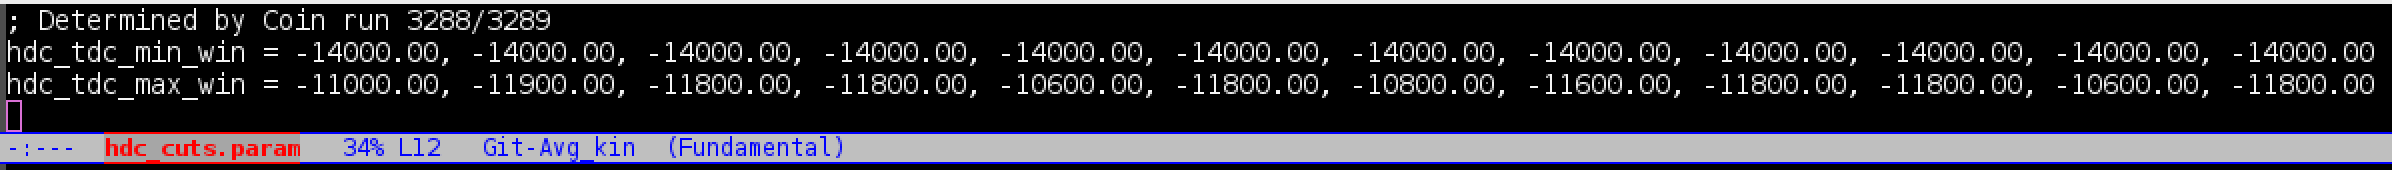
\includegraphics[scale=0.4]{plots/hdc_parm_cut.png}
  \caption{HMS DC TimeWindow cut parameter file.}
  \label{fig:hms_dc_parm_cut}
\end{figure}
\begin{figure}[H]
  \captionsetup{justification=raggedright,singlelinecheck=false}
  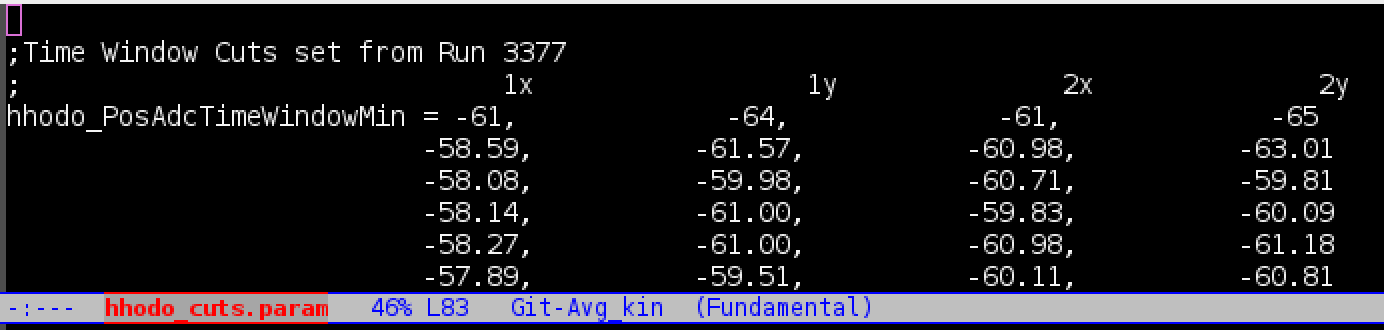
\includegraphics[scale=0.4]{plots/hhodo_parm_cut.png}
  \caption{HMS Hodo TimeWindow cut parameter file.}
  \label{fig:hms_hod_parm_cut}
\end{figure}
\begin{figure}[H]
  \captionsetup{justification=raggedright,singlelinecheck=false}
  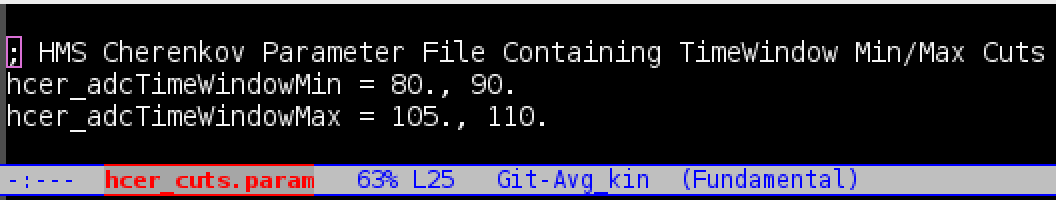
\includegraphics[scale=0.4]{plots/hcer_parm_cut.png}
  \caption{HMS Cherenkov TimeWindow cut parameter file.}
  \label{fig:hms_cer_parm_cut}
\end{figure}
\begin{figure}[H]
  \captionsetup{justification=raggedright,singlelinecheck=false}
  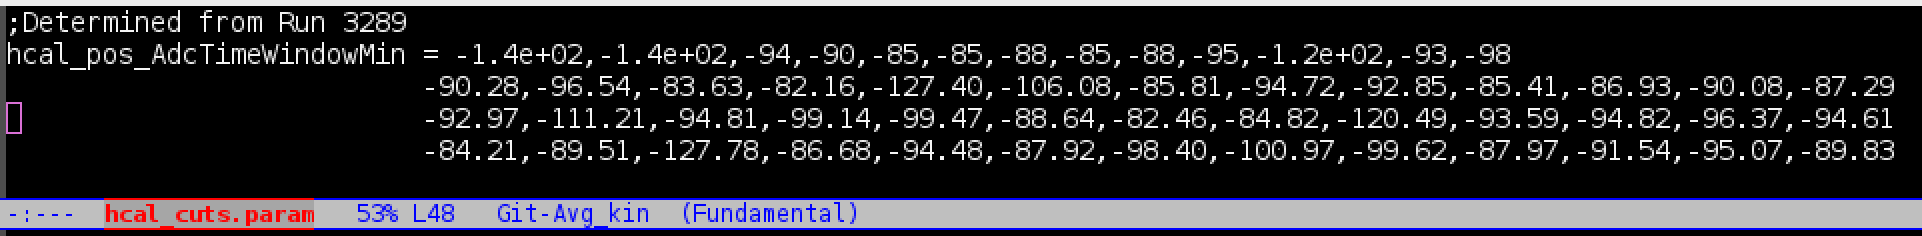
\includegraphics[scale=0.4]{plots/hcal_parm_cut.png}
  \caption{HMS Calorimeter TimeWindow cut parameter file.}
  \label{fig:hms_cal_parm_cut}
\end{figure}


\begin{figure}[H]
  \captionsetup{justification=raggedright,singlelinecheck=false}
  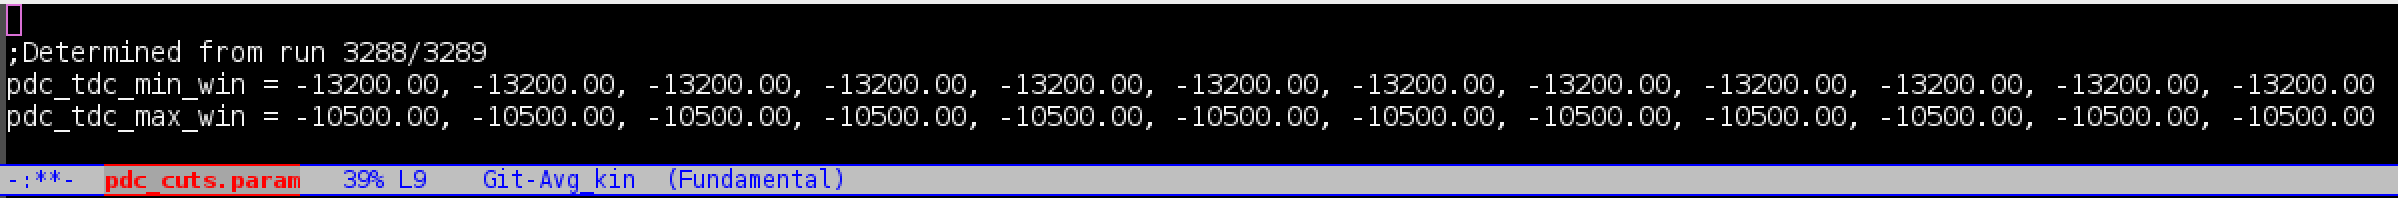
\includegraphics[scale=0.4]{plots/pdc_parm_cut.png}
  \caption{SHMS DC TimeWindow cut parameter file.}
  \label{fig:shms_dc_parm_cut}
\end{figure}
\begin{figure}[H]
  \captionsetup{justification=raggedright,singlelinecheck=false}
  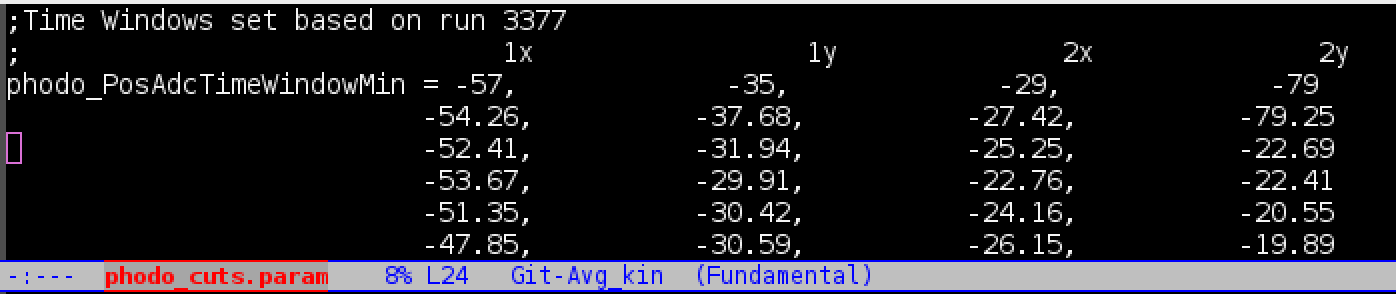
\includegraphics[scale=0.4]{plots/phodo_parm_cut.png}
  \caption{SHMS Hodo TimeWindow cut parameter file.}
  \label{fig:shms_hod_parm_cut}
\end{figure}
\begin{figure}[H]
  \captionsetup{justification=raggedright,singlelinecheck=false}
  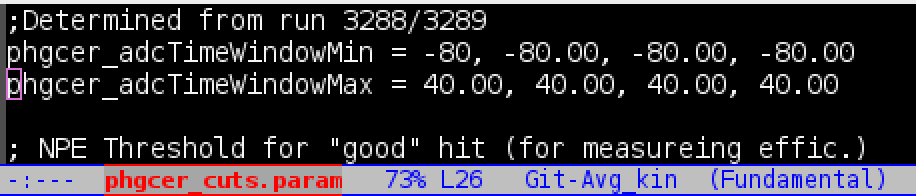
\includegraphics[scale=0.4]{plots/phgcer_parm_cut.png}
  \caption{SHMS HG Cherenkov TimeWindow cut parameter file.}
  \label{fig:shms_hgcer_parm_cut}
\end{figure}
\begin{figure}[H]
  \captionsetup{justification=raggedright,singlelinecheck=false}
  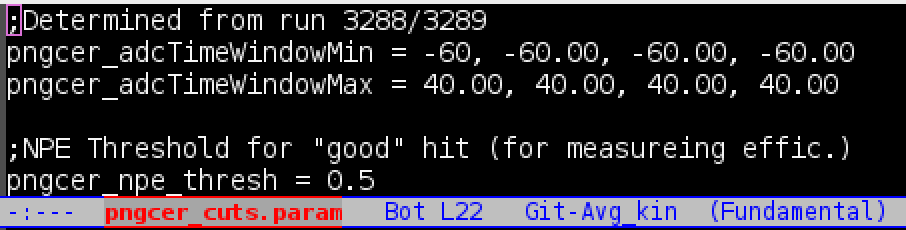
\includegraphics[scale=0.4]{plots/pngcer_parm_cut.png}
  \caption{SHMS NG Cherenkov TimeWindow cut parameter file.}
  \label{fig:shms_ngcer_parm_cut}
\end{figure}
\begin{figure}[H]
  \captionsetup{justification=raggedright,singlelinecheck=false}
  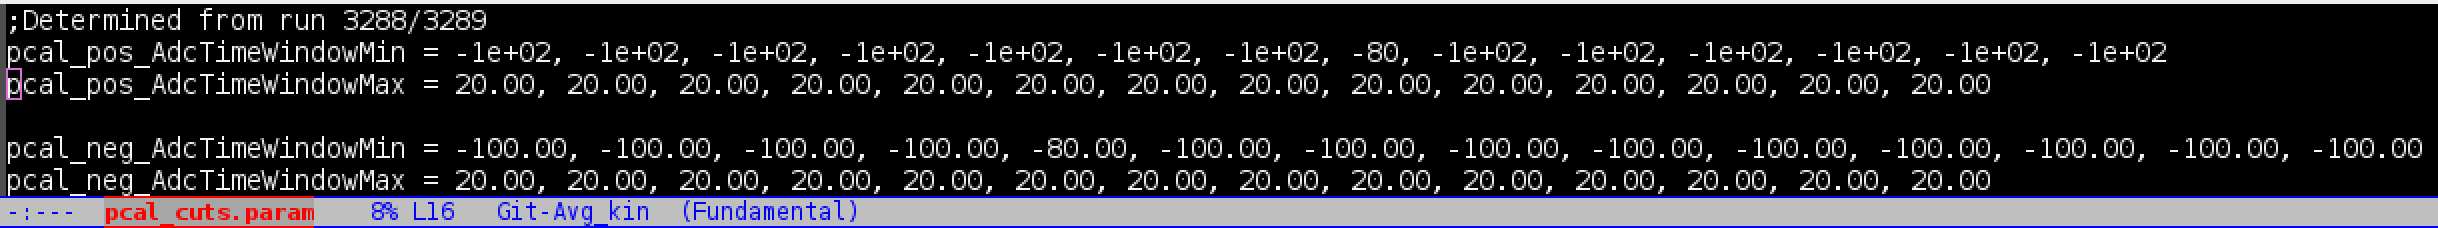
\includegraphics[scale=0.4]{plots/pprsh_parm_cut.png}
  \caption{SHMS PreShower TimeWindow cut parameter file.}
  \label{fig:shms_prsh_parm_cut}
\end{figure}
\begin{figure}[H]
  \captionsetup{justification=raggedright,singlelinecheck=false}
  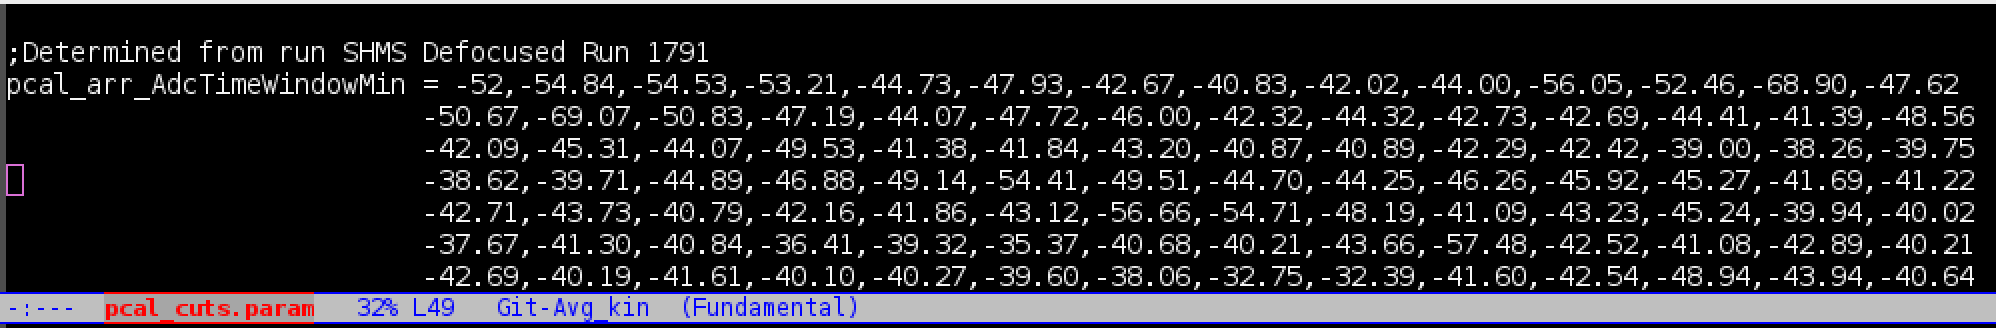
\includegraphics[scale=0.4]{plots/pcal_parm_cut.png}
  \caption{SHMS Calorimeter TimeWindow cut parameter file.}
  \label{fig:shms_cal_parm_cut}
\end{figure}

\end{appendices}
%Equations $\beta = \frac{v}{c}$.

%The general expression is
%\begin{equation} \label{eq1}
%\begin{split}
%A & = \frac{\pi r^2}{2} \\
% & = \frac{1}{2} \pi r^2
%\end{split}
%\end{equation}
%See Equation \ref{eq1}


%See Figure \ref{fig:Hodo}
%\begin{figure}[H]
%  \captionsetup{justification=raggedright,singlelinecheck=false}
%  \includegraphics[scale=0.3]{}
%  \caption{HMS Hodoscope 1X and 1Y Planes.}
%  \label{fig:Hodo}
%\end{figure}



% --------------------------------------------------------------
%     You don't have to mess with anything below this line.
% --------------------------------------------------------------
 
\end{document}
